% Copyright: CSCE240-001 - Fall 2016 - Group 7. All rights reserved.
% Date: 2016-11-30
%
% This is the base template file for the System Guide.
% First it contains the preamble
% Next, it contains a detailed description of the input and output of the program
% Sorted in topological order, it provides a listing for each class
% Finally, it traces an execution example to the most distal node.

\documentclass[letterpaper]{report}

\usepackage[numbers]{natbib}
\usepackage[hidelinks]{hyperref}

\renewcommand{\bibname}{References}
\renewcommand{\chaptername}{}
\usepackage{titlesec}
\titleformat{\chapter}[hang] 
{\normalfont\huge\bfseries}{\chaptertitlename\ \thechapter}{1em}{} 

\usepackage{listings}
\usepackage{tikz}
\usepackage{graphicx}
\usepackage{dcolumn}

% Used with permission from: https://www.overleaf.com/7261228mqbwdxppwphs
\definecolor{mygreen}{rgb}{0,0.6,0}
\definecolor{mygray}{rgb}{0.5,0.5,0.5}
\definecolor{mymauve}{rgb}{0.58,0,0.82}
\lstset{ %
  backgroundcolor=\color{white},   % choose the background color
  basicstyle=\footnotesize,        % size of fonts used for the code
  breaklines=true,                 % automatic line breaking only at whitespace
  captionpos=b,                    % sets the caption-position to bottom
  commentstyle=\color{mygreen},    % comment style
  escapeinside={\%*}{*)},          % if you want to add LaTeX within your code
  keywordstyle=\color{blue},       % keyword style
  stringstyle=\color{mymauve},     % string literal style
}

\newcolumntype{d}[1]{D{.}{\cdot}{#1} }
\DeclareGraphicsExtensions{.pdf,.png,.jpg}


\usepackage[intlimits]{mathtools}
\usepackage{amsfonts}
\usepackage{amsmath}
\usepackage{amsthm}
\usepackage{amssymb}
\usepackage{mathrsfs}


\usepackage{siunitx}

\usepackage[normalem]{ulem}
\usepackage{titling}

\title{Voter Simulation: System Guide}
\author{Hadrian Buckner \and Nicholas Grah \and Brian Griffin \and Peter Sanders \and Tahir Warid} 
\date{2016-12-01}

\begin{document}

\begin{titlepage}

{\centering
  {\scshape\Huge CSCE 240 \\ Intro. to Software Engineering\par}
  \vspace{1cm}
  {\scshape\LARGE \thetitle \par}
  \vspace{1cm}
  {\Large \theauthor \par}
  \vspace{1cm}
  {\scshape\large \thedate \par}
}

\vfill
\section*{Abstract}
The purpose of this program is to simulate voter wait-times and determine how many voting booths are necessary in any given precinct in order to ensure voters do not wait inordinately long amounts of time to cast their vote.
\vfill
\end{titlepage}

% Copyright: CSCE240-001 - Fall 2016 - Group 7. All rights reserved.
% Date: 2016-11-30
%
% This chapter describes the external data files for the program.
% That includes both those passed as arguments and those hard-coded.

\chapter{Input Files} \label{hxtk-input-files}

\section{Configuration File} \label{hxtk-config-file}

The configuration begins with a one-line header containing the following input data:

\begin{description}
\item[int] Some arbitrary random number seed.
\item[int$^+$] The length (in hours) of the election day.
\item[int$^+$] The best-guess mean service time of a voter in minutes.
\item[int$^+$] The minimum number of voters-per-precinct that will be supported by this simulation.
\item[int$^+$] The maximum number of voters-per-precinct that will be supported by this simulation.
\item[int$^+$] The maximum acceptable amount of time for a voter to wait.
\item[int$^+$] The number of iterations of the simulation to run. As more iterations are run, the data becomes asymptotically more ``complete'' with respect to consideration of outliers, but the execution time grows linearly.
\end{description}

The following line(s) should contain one $(1)$ more whitespace-delimited entries than the number of hours in the election day. These should be percent (\%) values and should sum to one hundred (100). The first value represents the fraction of voters who were already in line when polls opened. The subsequent values represent the fraction of voters arriving in each hour of the election day.

\section{Data File} \label{hxtk-data-file}

This file is hard-coded into the program. The program must be executed from two directories below a directory containing \texttt{dataallsorted.txt}. In other words, \texttt{../../dataallsorted.txt} must contain the data file.

This file should contain space-delimited integer values that represent voter service times in seconds. These values should be sorted in non-decreasing order.

\section{Precinct File} \label{hxtk-pct-file}

The precinct file contains the definitions of arbitrarily many precincts.

\vspace{0.5cm}

\emph{Note: The file must contain nothing but complete precincts. Any superfluous text, any incomplete entries, or any invalid entries will cause the program to exit.}

\vspace{0.5cm}

A Precinct is defined by the following information:

\begin{description}
\item[int] Precinct ID. This is a \emph{unique} numeric identifier for the precinct.
\item[text] Precinct Name. \emph{Note: Must NOT contain whitespace}.
\item[real] Precinct Turnout. The percentage of registered voters in a given precinct who actually voted.
\item[int$^+$] Actual number of voters.
\item[int$^+$] Number of voters expected.
\item[int$^+$] Expected rate of voters (voters per hour).
\item[int$^+$] Number of voting booths.
\item[real] Percent of minority voters.


% TODO(hxtk): I have no idea what these three stats mean.
%             Ngrah: you documented OnePct. Do you have anything to add?
\item[int$^+$] The last three items are used to set breakpoints. Detailed statistics are given as a histogram when the number of simulated voting booths is equal to the number given in these positions. Zero (0) is used to indicate the breakpoint is not used.
\item[int$^+$] 
\item[int$^+$] 
\end{description}

Only the number of expected voters and the precinct ID are used by the simulation. The other values are statistics that should be presented to the end user along with the simulation data.

\section{Output Files}

The last two arguments passed in the program call should be two file locations. The user executing this program must have write privileges at the specified location. The system must have on the order of megabytes of free space. Any files already existing at these locations will be overwritten.

% TODO(hxtk): create a chapter with label |hxtk-outfiles|
%             detailing the output of the program.
The first file is used for the output of the program. The second file will also contain the output of the program, but if debugging options are turned on at compile-time, it will also contain log information. See Chapter~\ref{hxtk-outfiles} for detailed information on their contents.

% Copyright: CSCE240-001 - Fall 2016 - Group 7. All rights reserved.
% Date: 2016-11-30
%
% This chapter the data written to the output files used by this program.

\chapter{Output Files} \label{hxtk-outfiles}

First, \texttt{MAIN} records the time and begins execution. Messages are printed to indicate the names of the output files.

Next, the configuration data is printed with the tag \texttt{CONFIG}. See \S\ref{hxtk-config-file} for more information.

\texttt{SIM} will be the next tag encountered. This is the \texttt{Simulation} class. It prints out the canonical string form of the \texttt{Precinct} being simulated. See \S\ref{ngrah-onepct-tostring} for more details on this string. As execution is passed off to this precinct, the next tag encountered is \texttt{OnePct}.

First, the canonical string form of the precinct is printed again. Next, the canonical string forms of the simulations for that precinct with one voting booth are printed. The number of simulations corresponds to the number of iterations specified in the configuration file. The canonical string form of a simulation may be found in Table~\ref{hxtk-canon-string-sim}. An example string follows, with superfluous whitespace omitted for the sake of space.

\vspace{1.0cm}

0 1 XXX00100 100 1 stations, mean/dev wait (mins) 0.43 0.95 toolong 0 0.00 0 0.00 0 0.00

\vspace{1.0cm}

This is repeated for as many iterations as were specified in the config file.

If the current number of voting booths was specified as a breakpoint in the Precinct File (See \S\ref{hxtk-pct-file}), a histogram is printed. One star on the histogram represents a computed value between one (1) and fifty (50) of voters. The histogram has a resolution of minutes and relates to the probability distribution function of voter wait time.

This, in turn, is repeated with incrementally more voting stations until there are no voters waiting too long.

Finally, this is repeated by \texttt{SIM} over the set of all precincts before returning execution to \texttt{MAIN}, printing the ending execution time.

\begin{table}[!h]
\caption{Canonical String Form of a Precinct Simulation}
\label{hxtk-canon-string-sim}
\begin{description}
\item[Simulation Number]
\item[Precinct ID]
\item[Precinct Name]
\item[Expected Voters]
\item[Number of Stations] This is followed by the text ``stations,''
\item[Mean time to vote (mins)] This is preceded by the text ``mean/dev wait (mins)''
\item[Standard Deviation of time to vote]
\item[Number of voters waiting too long] This is preceded by the text ``toolong''
\item[Percent of voters waiting too long]
\item[Number of voters waiting much too long] This is defined as ten (10) minutes longer than simply ``too long''
\item[Percent of voters waiting much too long]
\item[Number of voters waiting very much too long] This is defined as twenty (20) minutes longer than simply ``too long''
\item[Percent of voters waiting very much too long]
\end{description}
\end{table}

% Copyright: CSCE240-001 - Fall 2016 - Group 7. All rights reserved.
% Date: 2016-12-01
%
% This chapter describes the Main class.
% This class is the entry point for the voter simulation program. This class ensures the correct arguments were passed in, opens a Utils log file, and passes execution to the Simulation class.  

\chapter{Main}
The Main class is the entry point in the Voting Simulation program.
Main is responsible for gathering input and checking that arguments passed in are of the correct type.  Main also opens the Utils log file before passing executi0on to the Simulation class.

Main does not contain any member functions or variables.

Main supplies input data to the configuration class and the MyRandom class, and passes data to the Simulation class that will be used to create the voting precincts.

Once Input files have been properly handles, an instance of the Simulation class is created, and RunSimulation is called for that instance of simulation.





% Copyright: CSCE240-001 - Fall 2016 - Group 7. All rights reserved.
% Date: 2016-12-01
%
% This chapter describes the Simulation class
% This class begins performing the simulation by creating the voting precincts from the input file, and calling the RunSimulationPct function for each precinct.

\chapter{Simulation}
This class begins performing the simulation by creating the voting precincts from the input file, and calling the RunSimulationPct function for each precinct.

\section{General Functions}

\subsection{ReadPrecincts}
\begin{description}
\item[Parameters] Scanner& infile
\item[Returns] void
\item[Usage] Using a reference to the scanner reading from the input file, this function generates instances of OnePct and calls ReadData for that precinct, to populate it's member variables with values.
This continues until the scanner stops providing input.  These precints are stored in the pcts_ map.
\end{description}

\subsection{RunSimulation}
\begin{description}
\item[Parameters] const Configuration& config, MyRandom& random, ofstream& out_stream
\item[Returns] void
\item[Usage] This function iterates through the pcts_ map, and, if the precinct has an appropriate number of voters for the simulation, calls RunSimulationPct for that precinct.
\end{description}

\subsection{ToString}
\begin{description}
\item[Usage] Standard ToString function; Returns ToString of precincts stored in pcts_ map.
\end{description}

\section{Private Variables}

\begin{description}
\item[map<int, OnePct> pcts_] This map contains all instances of OnePct that will be used in the simulation.
\end{description}


% Copyright: CSCE240-001 - Fall 2016 - Group 7. All rights reserved.
% Date: 2016-11-30
%
% This chapter describes the OnePct class.
% This class is an instance of a single voting precinct for use in the simulation.

\chapter{OnePct}

The \texttt{OnePct} class is where the bulk of the work for this program happens.

Much of the data stored are statistics that are intended only to be presented to the user. The program does not use them anywhere as of this version.

This class depends upon the following public members of \texttt{Configuration}:

\begin{center}
\begin{lstlisting}[language=C++]
int election_day_length_hours_;
int election_day_length_seconds_;
int time_to_vote_mean_seconds_;
int wait_time_minutes_that_is_too_long_;
int number_of_iterations_;
vector<int> actual_service_times_;
double arrival_zero_;
vector<double> arrival_fractions_;
\end{lstlisting}
\end{center}

\section{ToString} \label{ngrah-onepct-tostring}

This defines the canonical string form of a Precinct. \emph{Note: this is not the same as the canonical string form of a precinct simulation as described in Table~\ref{hxtk-canon-string-sim}.} The Canonical String Form has the following whitespace-delimited fields:

\begin{description}
\item[ID] The integer-valued ID of the precinct. This must be unique within its batch.
\item[Name] This is a human-readable text identifier for the precinct. \emph{Note: since fields are whitespace delimited, this cannot contain whitespace}.
\item[Turnout] This is a percentage (\%) of voters who voted out of those who were registered for this precinct.
\item[Voters] This is the number of people registered to vote at this precinct.
\item[Expected Voters]
\item[Voter Rate] This is the mean number of voters expected per hour.
\item[Booths] This is the number of voting booths being used by the precinct.
\item[\% Minority] This is the percentage of minority voters out of all voters.
\item[HH] This is the string literal ``HH'' and serves as the opening delimiter for the set of histogram breakpoints.
\item[Break Point(s)] These are the number(s) of voting booths for which a histogram should be printed. There may be up to three (3).
\item[HH] This is the string literal ``HH'' and serves as the corresponding closing delimiter.
\end{description}

\section{ReadData}

\begin{center}
\begin{tabular}{l r}
Access & \texttt{public} \\
Return Type & \texttt{void} \\
Arguments & \texttt{Scanner\&}
\end{tabular}
\end{center}

This function accepts an open Scanner pointing at a \emph{complete} standard serialization of an \texttt{OnePct} object. This is further detailed in \S\ref{hxtk-pct-file}. If the Scanner is not opened or is not pointing at a valid input string, the program will crash.

\emph{No member function may be called until this function has completed.}

\section{RunSimulationPct}

\begin{center}
\begin{tabular}{l r}
Access & \texttt{public} \\
Return Type & \texttt{void} \\ \hline
Arguments & \texttt{const Configuration\&}\\
          & \texttt{MyRandom\&}\\
          & \texttt{ofstream\&}
\end{tabular}
\end{center}

This function runs a series of simulations and analyzes their outcomes based on the data contained in the Configuration object.

Beginning with the minimum value that cannot be rejected trivially, it uses incrementally more voting booths in the simulation until none of the voters are waiting too long. This is done by creating a randomized set of voters with \texttt{CreateVoters} and passing off the processing of the queue to \texttt{RunSimulationPct2}.

Once that is complete, \texttt{DoStatistics} is executed and if this number of voting booths was specified as a breakpoint, a histogram is printed.

\section{CreateVoters}

\begin{center}
\begin{tabular}{l r}
Access & \texttt{private} \\
Return Type & \texttt{void} \\ \hline
Arguments & \texttt{const Configuration\&}\\
          & \texttt{MyRandom\&}\\
          & \texttt{ofstream\&}
\end{tabular}
\end{center}

This uses random elements from a log-normal data set which should be made available to the program as specified in \S\ref{hxtk-data-file}.

First a set of voters waiting at the door on poll open is created, and then an exponential random distribution is used to bring in a given rate of voters for each hour.

\section{RunSimulationPct2}

\begin{center}
\begin{tabular}{l r}
Access & \texttt{private} \\
Return Type & \texttt{void} \\
Arguments & \texttt{int}
\end{tabular}
\end{center}

This function accepts the number of voting booths which should be used by the precinct and attempts to process the queue. This program must be run after \texttt{CreateVoters}

\section{DoStatistics}

\begin{center}
\begin{tabular}{l r}
Access & \texttt{private} \\
Return Type & \texttt{int} \\ \hline
Arguments & \texttt{int}\\
          & \texttt{const Configuration\&}\\
          & \texttt{int}\\
          & \texttt{map$<$int, int$>$}\\
          & \texttt{ofstream\&}
\end{tabular}
\end{center}

This function performs analysis of the data from the simulations. It must be called \emph{after} \texttt{RunSimulationPct2}. This function calls \texttt{ComputeMeanAndDev} and is the only valid context in which to do so.

\iffalse % BLOCK COMMENT
\section{Member Variables}

\begin{description}
\item[int pct\_expected\_voters\_] Number of voters expected to vote at this precinct.
\item[int pct\_expected\_per\_hour\_] Number of voters expected to vote at this precinct over a one hour period.
\item[double pct\_minority\_] Percentage of a precinct's voters who identified as a minority.
\item[string pct\_name\_] Name of an individual precinct.
\item[int pct\_number\_] Number assigned as an identifier to an individual precinct.
\item[double pct\_turnout\_] Percentage of the number of expected voters who showed up to vote at a precinct.  This is not used in calculations.
\item[int pct\_stations\_] Number of voting stations at a single precinct.
\item[int pct\_num\_voters\_]  Total number of voters who voted in a precinct.
\item[double wait\_dev\_seconds\_] The standard deviation of the wait times of the voters in a precinct in seconds.
\item[double wait\_mean\_seconds\_] The mean wait time of the voters in a precinct in seconds.
\item[set$<$int$>$ stations\_to\_histo\_] Set containing the number of voting stations used in the simulation.  This is meant to be displayed as part of a histogram of the data.
\item[vector$<$int$>$ free\_stations\_] Vector containing the stations not currently in use.  This is used in the RunSimulationPct2 function.
\item[multimap$<$int, OneVoter$>$ voters\_backup\_] This is a map containing all of the voters created by the CreateVoters function.  This map is populated before the real work of the simulation begins.
\item[multimap$<$int, OneVoter$>$ voters\_done\_voting\_] This map contains the voters who have already voted in the simulation. Voters in voters\_voting\_ are moved here when they have finished voting.
\item[multimap$<$int, OneVoter$>$ voters\_pending\_] This map begins as a copy of voters\_backu\_ before any voting has occurred. Voters are removed from this map as they finish voting, and are added voters\_done\_voting\_.
\item[multimap$<$int, OneVoter$>$ voters\_voting\_] This map contains voters who are currently at a voting station. Once a voter finishes voting, they are moved to voters\_done\_voting\_.
\end{description}


\section{General Functions}

\subsection{ReadData}
\begin{description}
\item[Parameters] Scanner\& infile
\item[Returns] void
\item[Usage] ReadData is passed in a reference to a scanner as input.  The data read by the scanner is used to provide values for the member variables of an instance of OnePct.
\end{description}


\subsection{RunSimulationPct}
\begin{description}
\item[Parameters] const Configuration\& config, MyRandom\& random, ofstream\& out\_stream
\item[Returns] void
\item[Usage] RunSimulationPct does the real work when simulating a single voting precinct.  This function generates voters, simulates voting for a precinct, and collects and stores the data from the simulation.
\end{description}
% TO-DO 

\subsection{ToString} \label{ngrah-onepct-tostring}
\begin{description}
\item[Parameters] none
\item[Returns] string s
\item[Usage] ToString Formats the information collected during the voting simulation, as well as the expected voters and expected voters per hour, and stores it to a string s.  String s is returned.
\item[Format] pct\_number  pct\_name\_ pct\_turnout\_  pct\_num\_voters\_  pct\_expected\_voters\_  pct\_expected\_per\_hour\_  pct\_stations\_ pct\_minority\_  "HH" Stations\_to\_histo\_ "HH"
\item[Example] 1  XXX00100 20.20      10101     100     235  8   10.30 HH    0 HH
\end{description}

\subsection{ToStringVoterMap}
\begin{description}
\item[Parameters] string label, multimap$<$int, OneVoter$>$ themap
\item[Returns] string s
\item[Usage] Takes a map of instances of voters as input.  This function iterates through the map of voters, calling ToString for each, and storing the returned string into string s.  This function then returns string s.
\end{description}


\section{General Private Functions}

\subsection{CreateVoters}
\begin{description}
\item[Parameters] const Configuration\& config, MyRandom\& random, ofstream\& out\_stream
\item[Returns] void
\item[Usage] This function is called by RunSimulationPct.  This function uses input from the config file, number of expected voters, and the random number generator to generate all the instances of voters used to simulate voting in a single precinct.
\end{description}

\subsection{DoStatistics}
\begin{description}
\item[Parameters] int iteration, const Configuration\& config, int station\_count, map$<$int, int$>$\& map\_for\_histo, ofstream\& out\_stream
\item[Returns] toolongcount (Number of voters who waited for too long)
\item[Usage] This function is called by RunSimulation.pct to determine the mean and standard deviation of vote times, and the number of voters who waited for too long at a single precinct.
\end{description}

\subsection{ComputeMeanAndDev}
\begin{description}
\item[Parameters] none
\item[Returns] void
\item[Usage] This function is called by the DoStatistics function.  This function calculates the mean and standard deviation of the wait times of voters for a single precinct.
\end{description}

\subsection{RunSimulationPct2}
\begin{description}
\item[Parameters] int stations\_count
\item[Returns] void
\item[Usage] This function is called by the RunSimulationPct function.  This function takes the number of open voting stations as input, and simulates moving the line of waiting voters through the voting stations.
\end{description}

\fi % END BLOCK COMMENT


% Copyright: CSCE240-001 - Fall 2016 - Group 7. All rights reserved.
% Date: 2016-12-01
%
% This chapter describes the OneVoter class.
% This class is an instance of a single voter to be used in the simulation program.

\chapter{OneVoter}
The OneVoter class is used to represent a single voter to be used in the voting simulation.  

\section{Constructor}
The Constructor for the OneVoter class takes in three integers as parameters.  These integers assign values to the Voter's sequence\_,time\_arrival\_seconds\_, and time\_vote\_duration\_seconds\_ variables.  The Time\_Start\_voting\_seconds\_ and which\_station variables are set to default values 0 and -1 by the constructor.

\section{General Functions}

\subsection{AssignStation}
\begin{description}
\item[Parameters] int station\_number, int start\_time\_seconds
\item[Returns] void
\item[Usage] This function takes in station\_number and Start\_time\_seconds, and uses the data to calculate which station the voter will use, total time spent voting, and total time spent waiting to vote.
\end{description}

\subsection{GetTimeDoneVoting}
\begin{description}
\item[Parameters] none
\item[Returns] returns the time spent voting as int
\item[Usage] calculates time spent voting by adding time\_start\_voting\_seconds\_ and time\_vote\_duration\_seconds\_.
\end{description}

\subsection{GetTimeInQ}
\begin{description}
\item[Parameters] none
\item[Returns] returns time spent in voting que as int
\item[Usage] calculates time spent in the voting que for a single voter by subtracting time\_arrival\_seconds\_ from time\_start\_voting\_seconds\_.
\end{description}

\subsection{GetTOD}
\begin{description}
\item[Parameters] int time\_in\_seconds
\item[Returns] Returns the time of day that a voter voted as a string.
\item[Usage] Uses time\_in\_seconds and offset\_hours to calculate when the voting took place.
\end{description}

\subsection{ConvertTime}
\begin{description}
\item[Parameters] int time\_in\_seconds
\item[Returns] returns a time as a string
\item[Usage] ues time in seconds to calculate time with hours, minutes, and seconds.  This function is called by GetTOD.
\end{description}

\subsection{ToString}
\begin{description}
\item[Usage] Standard ToString function for an instance of OneVoter.
\end{description}

\subsection{int time\_in\_seconds}
\begin{description}
\item[Usage] Returns a string of shortened variable names to act as a header for a table of voter data.
\end{description}

\section{Private Variables}

\begin{description}
\item[int sequence] Voters place in the que of voters.
\item[int time\_arrival\_seconds\_] Time voter arrived at polling station after station opened.
\item[int time\_done\_voting\_seconds\_] Time the voter has completed voting process.
\item[int time\_start\_voting\_seconds\_] The time a voter begins the voting process.
\item[int time\_vote\_duration\_seconds\_] Time a voter spends voting.
\item[int time\_waiting\_seconds\_] Time a voter spends waiting to vote.
\item[int which\_station\_] The voting station at which a voter votes.
\end{description}




% Copyright: CSCE240-001 - Fall 2016 - Group 7. All rights reserved.
% Date: 2016-12-01
%
% This file describes the purpose of the Configuration class.

\chapter{Configuration}

The Configuration class is dedicated to reading in the input files detailed in Chapter~\ref{hxtk-input-files}. All varaibles are publically accessible, so maintainers should take care to always pass references to this object as \texttt{const}.

This class is a \emph{Singleton}. A maintainer may wish to refactor it to this design pattern.

\begin{lstlisting}[language=C++]
static const int kDefaultSeed = 19;
static const int kDummyConfigInt = -111;
static const double kDummyConfigDouble = -22.22;

// This is the seed to be used for the Random Number Generator
int seed_ = kDefaultSeed;

int election_day_length_hours_ = kDummyConfigInt;
int election_day_length_seconds_ = kDummyConfigInt;
int time_to_vote_mean_seconds_ = kDummyConfigInt;
int max_expected_to_simulate_ = kDummyConfigInt;
int min_expected_to_simulate_ = kDummyConfigInt;
int wait_time_minutes_that_is_too_long_ = kDummyConfigInt;
int number_of_iterations_ = kDummyConfigInt;
vector<int> actual_service_times_;

// This is the percentage of voters already in line when pools opened.
double arrival_zero_ = kDummyConfigDouble;

// This array will contain |election_day_length_hours_| elements
// which shall correspond to the percentage of voters arriving
// during each hour of the election day
vector<double> arrival_fractions_;
\end{lstlisting}

% Copyright: CSCE240-001 - Fall 2016 - Group 7. All rights reserved.
% Date: 2016-12-1
%
% This chapter describes MyRandom class.
% This class is used to generate seudo-random numbers from a seed.


\chapter{MyRandom}
The MyRandom class is used to generate pseudo random numbrs from a seed provided.  The functions contained in MyRandom are used by this program to generate voter data.

\vspace{-1.0cm}

\section{Constructor}
The MyRandom class contains overloaded constructor functions. The first instance uses the integer 1 as the seed value, while the second takes an integer parameter value that is used for the seed. 
If a seed value is provided, MyRandom will use that value, but if a seed value is not provided, MyRandom will use a seed value of 1.

\section{RandomExponentialInt}
This function takes a double lambda as inpout, and returns an integer r.  The lambda is the is the lambda value of the exponentially distributed real numbers.  This function generates a double value based on the lambda constraint, rounds the double to the nearest integer, and returns this integer value.
This function is used in the Simulation Program to calculate the interval of voter arrival times.


\section{RandomNormal}
This function takes in doubles mean and dev for input, and generates a pseudo random number from a set with the provided mean and standard deviation.


\section{RandomUniformInt}
This function takes in two integers as parameters, describing the maximum and minimum values that can be generated.  This function returns a pseudo-randomly generated value that falls between the upper and lower limits provided.
In the Simulation Program, this function is used to calculate the time taken for a voter to finish voting.  This function works well time taking to vote must be greater than zero, and less than the maximum service time specifed in the config file.



% Copyright: CSCE240-001 - Fall 2016 - Group 7. All rights reserved.
% Date: 2016-11-30
%
% This traces the execution

\chapter{Execution Trace}

The execution begins at an entry point referred to here as \texttt{Main} and procedes, most distally, to \texttt{OneVoter} through a topology described in Figure~\ref{hxtk-exec-topology}.

Execution begins at \texttt{Main}. First, all variables used by \texttt{Main} are declared. First, boilerplate program entry is taken care of: Arguments are validated, files are opened, system state is recorded, etc.

An instance of \texttt{Configuration} is initialized from the corresponding stream, which is then closed.

\section{Configuration}

\texttt{Configuration} is a \emph{Singleton} collection of public variables that will be used throughout the program. It accepts an open stream for the configuration file, which should be of the format described in \S\ref{hxtk-config-file}. Next, a log-normal data set is read in by the same call. This stream is opened in context by the \texttt{Configuration::ReadConfiguration} function. \emph{NOTE: The program will crash if the file is not found.} The conditions for this file are given in \S\ref{hxtk-data-file}.

From here, execution returns to \texttt{Main} and procedes to \texttt{Simulation}.

\section{Simulation}

Simulation does very little work and exists only to group \texttt{Precinct}s into batches. Precincts are read in from a file first, then execution is passed off to each precinct in turn to run its simulation.

\section{OnePct}

This is the ``meat'' of the program. Execution first enters \texttt{OnePct} at \texttt{RunSimulationPct}.

A simulation runs through a day of voting in order to determine the number of voting booths required to handle voters efficiently. The purpose of \texttt{OnePct::RunSimulationPct} is to regulate the number of voting booths being simulated. Given a mean voting time in seconds ($MVT$) and a number of voters ($NV$) on an election day ($L$) hours long, the initial number of voting booths ($VB_0$) is given by Equation~\ref{hxtk-init-booths} below.

\begin{equation} \label{hxtk-init-booths}
VB_0 = \begin{cases}
  \lfloor \frac{MVT \times NV}{3600\times L} \rfloor & MVT \times NV \ge 3600\times L \\
  1 & \text{otherwise}
\end{cases}
\end{equation}

Beginning with this number and iterating upwards until no voters are waiting ``too long,'' the program runs the number of iterations indicated by \S\ref{hxtk-config-file}. After all iterations have run, a histogram is printed if this number of voting machines is a breakpoint number for this precinct.

\subsection{CreateVoters}

Each single iteration consists of three parts. First, voters are created. This includes a set of voters waiting at the door when the polls open and exponential random voters at the hourly rates indicated by the configuration file.

\subsection{RunSimulationPct2}

Next, simulation is passed off to another function. This manages the processing of voters through the queue.

\subsection{DoStatistics}

Finally, some statistics are run to determine if any voters waited too long, among other things.

\begin{figure}
\begin{center}
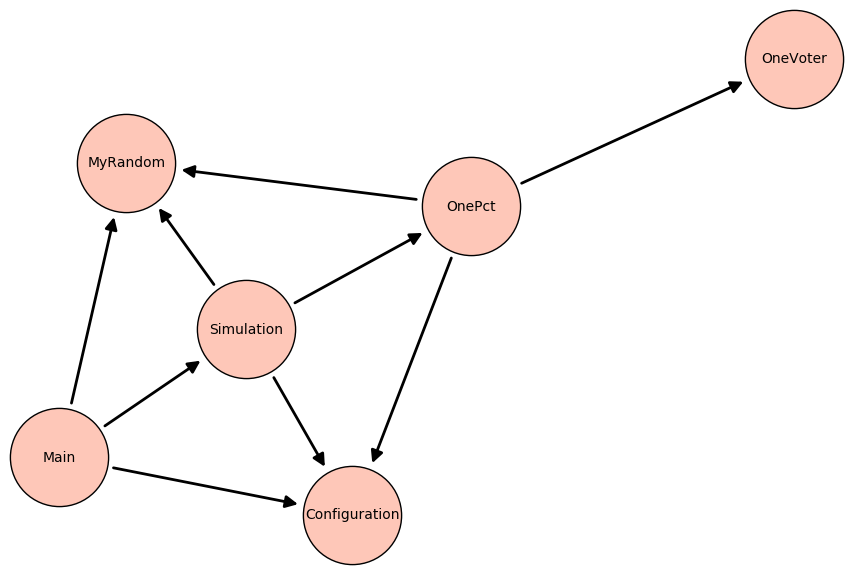
\includegraphics[width=\textwidth]{execution_topology}
\end{center}
\caption{Execution Topology by Class} \label{hxtk-exec-topology}
\end{figure}

\end{document}
